\subsection{RQ5: How does static-analysis feedback affect the ability of language models to detect errors in generated code?}

\begin{table*}[htbp]
\centering
\caption{Detection results with static-analysis feedback, compared with the no-feedback setting of RQ2. Values are percentages and the value in parentheses is the change relative to RQ2.}
\label{tab:rq5_detection_delta}
\begin{tabular}{lrrrrrr}
\toprule
\textbf{Model} & \textbf{Acc} & \textbf{MF1} & \textbf{CR} & \textbf{FR} & \textbf{RR} & \textbf{SR} \\
\midrule
\multicolumn{7}{l}{\emph{General-purpose models}} \\
\midrule
Muse Glimmer 30B & \scorecell{79}{79 (+6)} & \scorecell{71}{71 (+17)} & \scorecell{89}{89 (+6)} & \scorecell{58}{58 (+3)} & \scorecell{25}{25 (-2)} & \scorecell{100}{100 (+47)} \\
Gemma 4 31B & \scorecell{77}{77 (+4)} & \scorecell{66}{66 (+18)} & \scorecell{87}{87 (+3)} & \scorecell{56}{56 (+6)} & \scorecell{23}{23 (-1)} & \scorecell{100}{100 (+22)} \\
Qwen 3.8 27B & \scorecell{69}{69 (+7)} & \scorecell{56}{56 (+13)} & \scorecell{73}{73 (+10)} & \scorecell{69}{69 (-6)} & \scorecell{9}{9 (-4)} & \scorecell{100}{100 (+35)} \\
Qwen 2.5 Coder 7B & \scorecell{37}{37 (-26)} & \scorecell{47}{47 (+13)} & \scorecell{24}{24 (-49)} & \scorecell{89}{89 (+43)} & \scorecell{8}{8 (+5)} & \scorecell{100}{100 (+82)} \\
Qwen 2.5 Coder 32B & \scorecell{43}{43 (-18)} & \scorecell{50}{50 (+9)} & \scorecell{44}{44 (-27)} & \scorecell{47}{47 (+9)} & \scorecell{9}{9 (-3)} & \scorecell{100}{100 (+24)} \\
Qwen 3 Coder 30B & \scorecell{52}{52 (-8)} & \scorecell{46}{46 (+9)} & \scorecell{46}{46 (-18)} & \scorecell{86}{86 (+20)} & \scorecell{4}{4 (-5)} & \scorecell{100}{100 (+78)} \\
Ornith 1.5 35B & \scorecell{59}{59 (+2)} & \scorecell{52}{52 (+16)} & \scorecell{55}{55 (-1)} & \scorecell{84}{84 (+6)} & \scorecell{8}{8 (+0)} & \scorecell{100}{100 (+62)} \\
Devstral Small 2 24B & \scorecell{56}{56 (+2)} & \scorecell{53}{53 (+15)} & \scorecell{54}{54 (-1)} & \scorecell{71}{71 (+7)} & \scorecell{11}{11 (-6)} & \scorecell{100}{100 (+65)} \\
GLM 4.7 Flash 30B & \scorecell{46}{46 (-4)} & \scorecell{45}{45 (+7)} & \scorecell{37}{37 (-13)} & \scorecell{88}{88 (+24)} & \scorecell{9}{9 (-17)} & \scorecell{100}{100 (+6)} \\
Gemma 4 E2B IT & \scorecell{50}{50 (+2)} & \scorecell{49}{49 (+16)} & \scorecell{48}{48 (+0)} & \scorecell{68}{68 (+3)} & \scorecell{10}{10 (-6)} & \scorecell{94}{94 (+88)} \\
Gemma 4 E4B IT & \scorecell{46}{46 (+0)} & \scorecell{52}{52 (+15)} & \scorecell{35}{35 (-3)} & \scorecell{93}{93 (+6)} & \scorecell{20}{20 (-11)} & \scorecell{100}{100 (+50)} \\
Gemma 3 4B IT & \scorecell{36}{36 (-2)} & \scorecell{46}{46 (+19)} & \scorecell{25}{25 (-5)} & \scorecell{83}{83 (+1)} & \scorecell{8}{8 (-3)} & \scorecell{94}{94 (+88)} \\
Gemma 3 4B & \scorecell{36}{36 (+3)} & \scorecell{47}{47 (+24)} & \scorecell{24}{24 (+2)} & \scorecell{82}{82 (-3)} & \scorecell{9}{9 (+3)} & \scorecell{100}{100 (+82)} \\
GPT-OSS 20B & \scorecell{31}{31 (+6)} & \scorecell{50}{50 (+11)} & \scorecell{26}{26 (+8)} & \scorecell{52}{52 (-4)} & \scorecell{27}{27 (-6)} & \scorecell{100}{100 (+27)} \\
\midrule
\multicolumn{7}{l}{\emph{Fine-tuned models}} \\
\midrule
Best Acc & \scorecell{77}{77 (+0)} & \scorecell{68}{68 (+17)} & \scorecell{85}{85 (+0)} & \scorecell{65}{65 (-4)} & \scorecell{19}{19 (-9)} & \scorecell{100}{100 (+88)} \\
Weighted MF1 & \scorecell{76}{76 (+2)} & \scorecell{68}{68 (+14)} & \scorecell{79}{79 (+4)} & \scorecell{75}{75 (-3)} & \scorecell{20}{20 (-13)} & \scorecell{100}{100 (+31)} \\
Balanced Acc & \scorecell{67}{67 (-1)} & \scorecell{36}{36 (-2)} & \scorecell{71}{71 (-3)} & \scorecell{71}{71 (+5)} & \scorecell{10}{10 (-5)} & \scorecell{0}{0 (+0)} \\
Balanced MF1 & \scorecell{61}{61 (-3)} & \scorecell{56}{56 (+20)} & \scorecell{62}{62 (-7)} & \scorecell{74}{74 (+8)} & \scorecell{7}{7 (-7)} & \scorecell{81}{81 (+81)} \\
\midrule
\multicolumn{7}{l}{\emph{Large models}} \\
\midrule
DeepSeek V4.1 Flash & \scorecell{76}{76 (+1)} & \scorecell{64}{64 (+13)} & \scorecell{88}{88 (-2)} & \scorecell{55}{55 (+4)} & \scorecell{10}{10 (-5)} & \scorecell{100}{100 (+65)} \\
MiMo V2.5 & \scorecell{47}{47 (-4)} & \scorecell{47}{47 (+8)} & \scorecell{37}{37 (-10)} & \scorecell{90}{90 (+10)} & \scorecell{9}{9 (-13)} & \scorecell{100}{100 (+4)} \\
\bottomrule
\end{tabular}
\end{table*}

In this research question, we evaluated how error-detection behavior changes when we add content from static tool feedback. This study seeks to understand how models utilize this additional content and whether it can harm model analysis. For this task, we followed the same process as the first classification stage, adding only feedback from the compiler and Pyright. Table ~\ref{tab:rq5_detection_delta} presents all the performance data of these models in this task, including the trained models.

The main effect is evident in \emph{Syntax Error} detection: after feedback, 16 of the 20 evaluated models achieved more than 94\% detection, with 14 reaching 100\%. The impact was significant, especially for models that increased the rate by 78 p.p. or more compared with the analysis without these tools. In other words, with these tools, the models began to show plausible detection performance, although the detection was performed by the tool, not the model. This analysis shows that models can be less reliable when they use tool output as ground truth.

The only caveat is that the analysis is based on models that, in their training set, showed reduced classification of this class. In the optimization strategy that sought the greatest accuracy gain, the model showed low sensitivity to the response, indicating great difficulty in generalizing between types, while the model trained with the objective of optimization aiming for a greater balance between classes obtained better performance; however, even so, it did not respond correctly in all classes.

\begin{figure}[htbp]
\centering
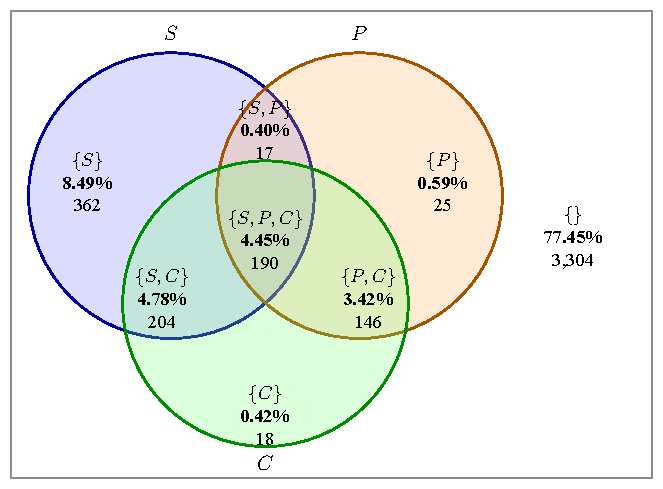
\includegraphics[width=\columnwidth]{figures/rq5_runtime_venn.pdf}
\caption{Runtime Error detection across 18 SLM configurations (4,266 matched judgments). $S$: SLM without feedback; $P$: Pyright; $C$: SLM with feedback. Percentages use all matched judgments; circle areas are not proportional.}
\label{fig:runtime_venn}
\end{figure}

In Runtime Error detection, the opposite was true: with an average variation of -5.04 p.p., progression occurred in only 2 cases; in the other 16, regression. This main deviation can be associated with Pyright because, with performance inferior to the models' own detection, the models largely accepted the tool's evaluation. This is visible in the Venn Diagram in Figure~\ref{fig:runtime_venn}, where the largest subset of detections (8.49\% of cases) came only from the model, without adding the tool's content.

In some scenarios, the model did not accept positive feedback from the tool: Qwen 3 Coder 30B rejected 13 validations from the tool, while GLM 4.7 Flash showed a clearer sign of regression, losing 17 pp, without any scenario in which it pointed out an error beyond what had already been pointed out by the tool.

Although the feedback applied to only two classes, it affected the classification of the others. Positively, we observed that Average Recall increased by 6.66 pp among the models in detecting \emph{Functional Errors}, while \emph{Correct} decreased, with average Recall reduced by 5.19 pp. This drop can be explained by the tool's false positives: of the 114 cases previously marked as \emph{Correct}, only 2 remained correctly classified after the tool generated a false positive.
